\documentclass[10.5pt]{article}
\usepackage{amsmath,amssymb,amsthm}
\usepackage{listings}
\usepackage{graphicx}
\usepackage[shortlabels]{enumitem}
\usepackage{tikz}
\usepackage[margin=1in]{geometry}
\usepackage{fancyhdr}
\usepackage{epsfig} %% for loading postscript figures
\usepackage{amsmath}
\usepackage{float}
\usepackage{amssymb}
\usepackage{caption}
\usepackage{subfigure}
\usepackage{graphics}
\usepackage{titlesec}
\usepackage{mathrsfs}
\usepackage{amsfonts}
\usepackage{indentfirst}
\usepackage{fancybox}
\usepackage{tikz}
\usepackage{algorithm}
\usepackage{algcompatible}
\usepackage{fontspec}
\usepackage{listings}
\usepackage{xcolor}      %代码着色宏包
\usepackage{CJK}         %显示中文宏包
\lstset{
    basicstyle=\tt,
    %行号
    numbers=left,
    rulesepcolor=\color{red!20!green!20!blue!20},
    escapeinside=``,
    xleftmargin=2em,xrightmargin=2em, aboveskip=1em,
    %背景框
    framexleftmargin=1.5mm,
    frame=shadowbox,
    %背景色
    backgroundcolor=\color[RGB]{245,245,244},
    %样式
    keywordstyle=\color{blue}\bfseries,
    identifierstyle=\bf,
    numberstyle=\color[RGB]{0,192,192},
    commentstyle=\it\color[RGB]{96,96,96},
    stringstyle=\rmfamily\slshape\color[RGB]{128,0,0},
    %显示空格
    showstringspaces=false
}

\renewcommand{\baselinestretch}{1.2}%Adjust Line Spacing
%\geometry{left=2.0cm,right=2.0cm,top=2.0cm,bottom=2.0cm}% Adjust Margins of the File
\usepackage{tikz-qtree}
\usetikzlibrary{graphs}
\usetikzlibrary{arrows.meta}
\tikzset{every tree node/.style={minimum width=2em,draw,circle},
	blank/.style={draw=none},
	edge from parent/.style=
	{draw,edge from parent path={(\tikzparentnode) -- (\tikzchildnode)}},
	level distance=1.2cm}
\setlength{\parindent}{0pt}
%\setlength{\parskip}{5pt plus 1pt}
\setlength{\headheight}{13.6pt}
\newcommand\question[2]{\vspace{.25in}\hrule\textbf{#1: #2}\vspace{.5em}\hrule\vspace{.10in}}
\renewcommand\part[1]{\vspace{.10in}\textbf{(#1)}}
%\newcommand\algorithm{\vspace{.10in}\textbf{Algorithm: }}
\newcommand\correctness{\vspace{.10in}\textbf{Correctness: }}
\newcommand\runtime{\vspace{.10in}\textbf{Running time: }}
\pagestyle{fancyplain}
% Create horizontal rule command with an argument of height
\newcommand{\horrule}[1]{\rule{\linewidth}{#1}}
% Set the title here
\title{
	\normalfont \normalsize
	\textsc{ShanghaiTech University} \\ [25pt]
	\horrule{0.5pt} \\[0.4cm] % Thin top horizontal rule
	\huge CS101 Algorithms and Data Structures\\ % The assignment title
	\LARGE Fall 2021\\
	\LARGE Homework 10\\
	\horrule{2pt} \\[0.5cm] % Thick bottom horizontal rule
}
% wrong usage of \author, never mind
\author{}
\date{Due date: 23:59, December 12, 2020}

% set the header and footer
\pagestyle{fancy}
\lhead{CS101 Algorithms and Data Structures}
\chead{Homework 10}
\rhead{Due date: 23:59, December 12, 2020}
\cfoot{\thepage}
\renewcommand{\headrulewidth}{0.4pt}
\newtheorem{Q}{Question}
% special settings for the first page
\fancypagestyle{firstpage}
{
	\renewcommand{\headrulewidth}{0pt}
	\fancyhf{}
	\fancyfoot[C]{\thepage}
}

% Add the support for auto numbering
% use \problem{title} or \problem[number]{title} to add a new problem
% also \subproblem is supported, just use it like \subsection
\newcounter{ProblemCounter}
\newcounter{oldvalue}
\newcommand{\problem}[2][-1]{
	\setcounter{oldvalue}{\value{secnumdepth}}
	\setcounter{secnumdepth}{0}
	\ifnum#1>-1
	\setcounter{ProblemCounter}{0}
	\else
	\stepcounter{ProblemCounter}
	\fi
	\section{Problem \arabic{ProblemCounter}: #2}
	\setcounter{secnumdepth}{\value{oldvalue}}
}
\newcommand{\subproblem}[1]{
	\setcounter{oldvalue}{\value{section}}
	\setcounter{section}{\value{ProblemCounter}}
	\subsection{#1}
	\setcounter{section}{\value{oldvalue}}
}

\setmonofont{Fira Code}
\definecolor{blve}{rgb}{0.3372549 , 0.61176471, 0.83921569}
\definecolor{gr33n}{rgb}{0.29019608, 0.7372549 , 0.64705882}
\makeatletter
\lst@InstallKeywords k{class}{classstyle}\slshape{classstyle}{}ld
\makeatother
\lstset{language=C++,
	basicstyle=\ttfamily,
	keywordstyle=\color{blve}\ttfamily,
	stringstyle=\color{red}\ttfamily,
	commentstyle=\color{green}\ttfamily,
	morecomment=[l][\color{magenta}]{\#},
	classstyle = \bfseries\color{gr33n}, 
	tabsize=4
}

\begin{document}
\maketitle
\thispagestyle{firstpage}
%\newpage
\vspace{3ex}

\begin{enumerate}
	\item Please write your solutions in English.

	\item Submit your solutions to gradescope.com.

	\item Set your Full Name to your Chinese name and your STUDENT ID correctly in Account Settings.

	\item If you want to submit a handwritten version, scan it clearly. Camscanner is recommended.

	\item When submitting, match your solutions to the according problem numbers correctly.

	\item No late submission will be accepted.

	\item Violations to any of above may result in zero score.
\end{enumerate}
\newpage

%---------------------------------------------------------
\question{1}{(4*2') Multiple Choices}

Each question has one or more correct answer(s). Select all the correct answer(s). For each question, you get $0$ point if you select one or more wrong answers, but you get $1$ point if you select a non-empty subset of the correct answers.\\
\textit{Note that you should write you answers of section 1 in the table below.}
\begin{table}[htbp]
	\begin{tabular}{|p{2cm}|p{2cm}|p{2cm}|p{2cm}|}
		\hline
		Question 1 & Question 2 & Question 3 & Question 4 \\
		\hline
		B D        & B C        & B C        & C          \\
		\hline
	\end{tabular}
\end{table}

\begin{Q}
	Which of the followings are true?
	\begin{enumerate}[(A)]
		\item Like Dijkstra's algorithm, Floyd-Warshall algorithm cannot work with any graph with negative weight edge.
		\item \textbf{With a simple optimization}, applying Floyd-Warshall algorithm to an \textbf{undirected} graph of N nodes just needs to take \textbf{about} half of the time of applying it to a \textbf{directed} graph of N nodes. (Do not need to be strictly 1/2)
		\item If a graph has non-negative edges, it is always preferable to run the Floyd-Warshall algorithm to solve an all-pair shortest path problem than call |V| times Dijkstra's algorithm.
		      % 		same graph
		\item In Floyd-Warshall algorithm, we always have the shortest path between any pair of vertexes which only passes through the vertex set $\{v_m|m\leq k\}$ after k iterations of the outmost loop.
	\end{enumerate}
\end{Q}

\begin{Q}
	Which of the followings are true?
	\begin{enumerate}[(A)]
		\item For A* search algorithm, if the heuristic is admissible, then it is also consistent.
		\item For A* search algorithm, if the heuristic is consistent, then it is also admissible.
		\item For A* search algorithm with admissible and consistent heuristic, heuristic $h_a(x)$ is always better than $h_b(x)$ if $\forall x: h_a(x) \geq h_b(x)$.
		\item For A* search algorithm with admissible and consistent heuristic, heuristic $h_a(x)$ is always better than $h_b(x)$ if $\forall x: h_a(x) \leq h_b(x)$.
	\end{enumerate}
\end{Q}

\begin{Q}
	Which of the followings are true?
	\begin{enumerate}[(A)]
		\item For A* tree search algorithm, it will always return an optimal solution if it exists.
		\item For A* tree search algorithm with admissible heuristic, it will always return an optimal solution if it exists.
		\item For A*  tree search algorithm with consistent heuristic, it will always return an optimal solution if it exists.
		\item None of the above.
	\end{enumerate}
\end{Q}

\begin{Q}
	Which of the followings are true?
	\begin{enumerate}[(A)]
		\item For A* graph search algorithm, it will always return an optimal solution if it exists.
		\item For A* graph search algorithm with admissible heuristic, it will always return an optimal solution if it exists.
		\item For A* graph search algorithm with consistent heuristic, it will always return an optimal solution if it exists.
		\item None of the above.
	\end{enumerate}
\end{Q}

%---------------------------------------------------------
\question{2}{(6') Floyd-Warshall algorithm}
\begin{Q}
	Consider the following implementation of the Floyd-Warshall algorithm. Assume $w_{ij}=\infty$ where there is no edge between vertex $i$ and vertex $j$, and assume $w_{ii}=0$ for every vertex $i$. Add some codes in the blank lines to detect whether there is negative cycles in the graph. (You may not use all blank lines.)
	\lstset{language=C++}
	\begin{lstlisting}    
bool detectNegCycle(int graph[][V]) 
{ 
    int dist[V][V], i, j, k; 
   
    for (i = 0; i < V; i++) 
        for (j = 0; j < V; j++) 
            dist[i][j] = graph[i][j]; 
   
    for (k = 0; k < V; k++) { 
        for (i = 0; i < V; i++) { 
            for (j = 0; j < V; j++) { 
                if (dist[i][k] + dist[k][j] < dist[i][j]) 
                        dist[i][j] = dist[i][k] + dist[k][j]; 
            } 
        } 
    } 
    
    for (k = 0; k < V; k++) {
        if (dist[k][k] < 0)
            return true;
    }
            
    return false;  
} 

\end{lstlisting}

\end{Q}


\newpage
%---------------------------------------------------------
\question{3}{(4'+4') A* Graph Search}
Here is the pseudocode of Graph Search. We can take $fringe$ as the priority queue.
\begin{figure}[htbp]
	\centerline{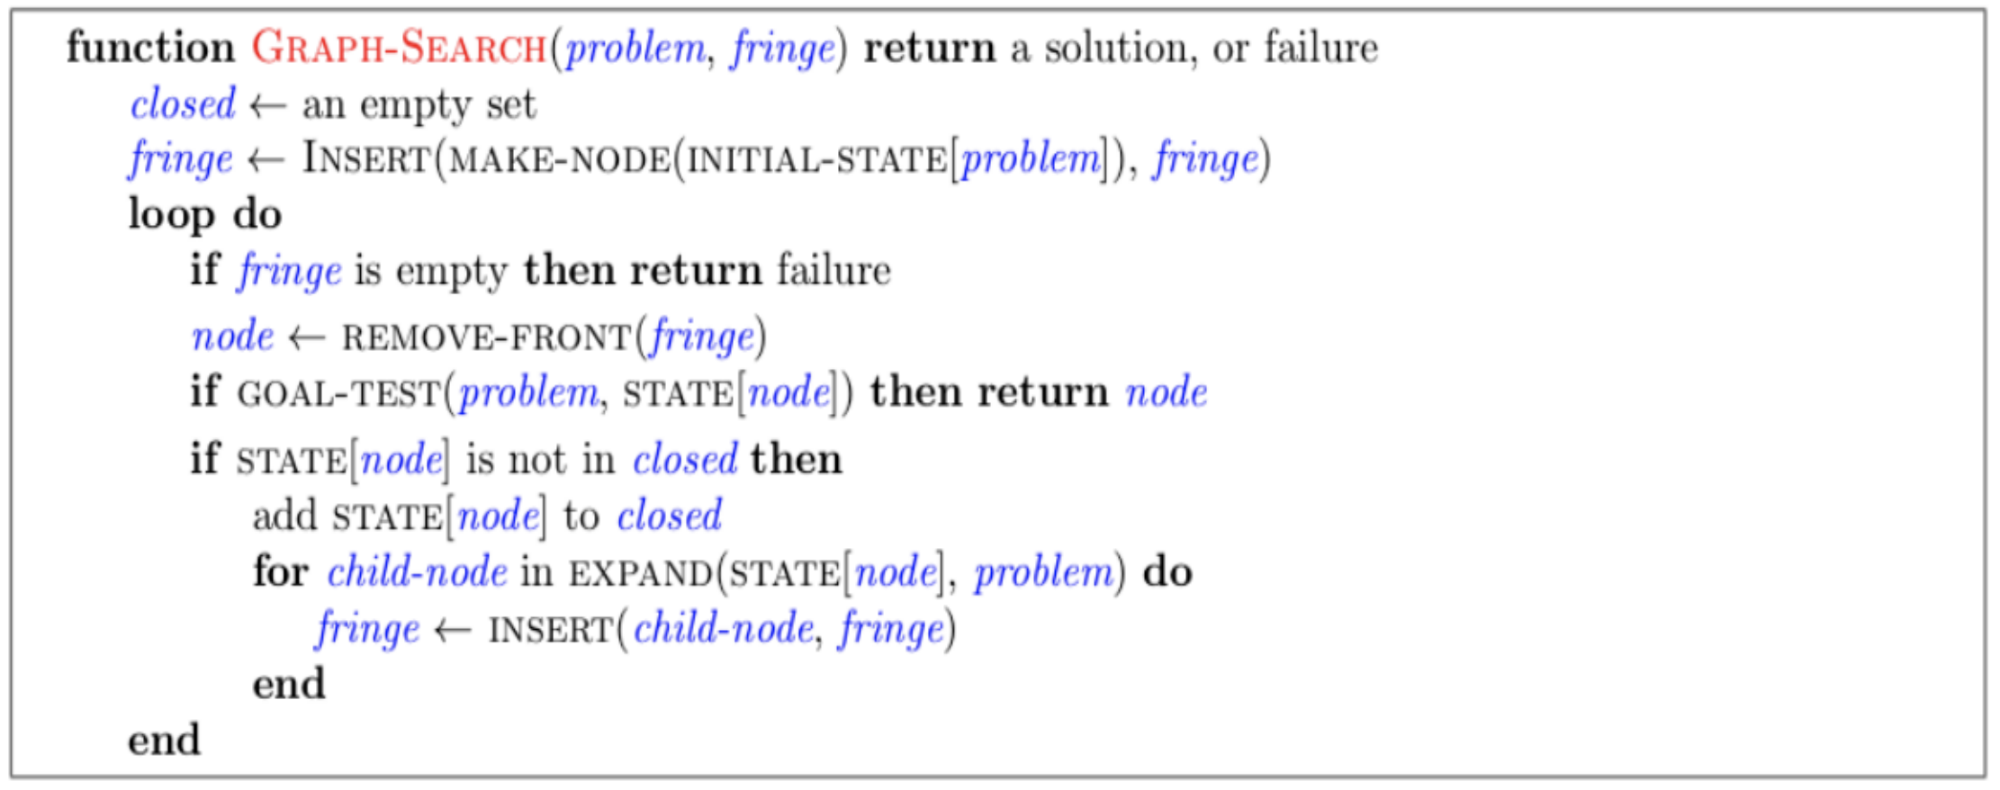
\includegraphics[scale=0.20]{graph-search.png}}
	\label{fig1}
\end{figure}

Consider A* graph search on the graph below. Edges are labeled with costs and vertices are labeled with heuristic values. Assume that ties are broken alphabetically (so a partial plan S->X->A would be expanded before S->X->B and S->A->Z would be expanded before S->B->A).
\begin{figure}[htbp]
	\centerline{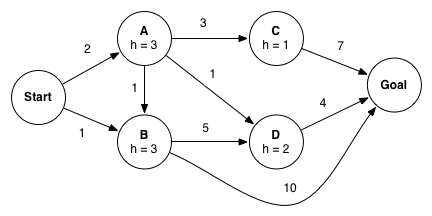
\includegraphics[scale=0.66]{a_star_graph.png}}
	\label{fig3}
\end{figure}

\begin{Q}
	In what order are vertices expanded by A* graph search? Write the expanding sequence below. (e.g. Start, A, B, C, D, Goal)\\
\end{Q}
Start, B, A, D, C, Goal\\
\begin{Q}
	What path does A* graph search return? Write the path below. (e.g. Start --> A --> C --> Goal)
\end{Q}

Start --> A --> D --> Goal\\


\newpage

\question{4}{(4*2') A*-CSCS}
After seeing the A* search algorithm, in this question we explore a new search procedure using a dictionary for the closed set, A∗ graph search with Cost Sensitive Closed Set (A*- CSCS).

\begin{figure}[htbp]
	\centerline{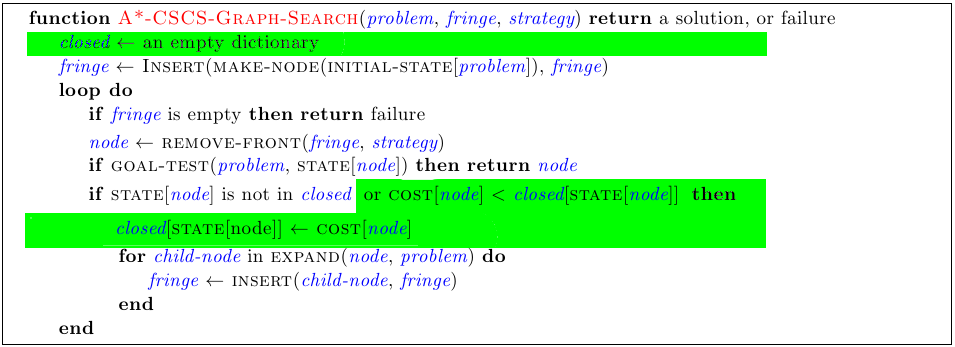
\includegraphics[scale=0.45]{a-star-cscs.png}}
	\label{fig2}
\end{figure}

Rather than just inserting the last state of a node into the closed set, we now store the last state paired with the cost of the node. Whenever A*- CSCS considers expanding a node, it checks the closed set. Only if the last state is not a key in the closed set, or the cost of the node is less than the cost associated with the state in the closed set, the node is expanded.

For the following questions, if you think the statement is correct, give a \textbf{brief} proof or explanation, if you think the statement is wrong, give a \textbf{brief} counter-example or explanation.\\
\\
\textcolor{purple}{
	\textbf{Notations: }\\
	Let $f(n)$ be the actual cost of the optimal path $P$ start from $s$, end with $t$ and pass through $n$. \\
	Let $g(n)$ be the actual cost of optimal path from $s$ to $n$.\\
	Let $h(n)$ be the actual cost of optimal path from $n$ to $t$.\\
	Then, $f(n) = g(n) + h(n)$.\\
	Let $\hat g(n)$ be an estimate of $g(n)$ and $\hat h(n)$ be an esitamte of $h(n)$.\\
	By defination, $\hat g(n) \ge g(n)$.\\
	An estimate of $f(n)$ is $\hat f(n) = \hat g(n) + \hat h(n)$.\\
	$COST[node]$ equals to $\hat g(node)$.\\
	$A^*$ strategy always remove node with smallest $\hat f(node)$ in the fringe.\\
	An admissible heuristic means $\hat h(n) \le h(n)$ for all $n$ in the $problem$.\\
	An consistent heuristic means \(\hat h(n) + h(m, n) \ge \hat h(m)\).\\
	The $A^*$ will terminate as soon as $t$ is removed from $fringe$.
}\\
\pagebreak
\begin{Q}
	The A*-CSCS algorithm with an admissible heuristic will find an optimal solution.
\end{Q}
Yes.\\
(Please refer to the notations on the top of this section.)\\
\textbf{Lemma 1:} If $t$ is not in $closed$, and for any optimal path $T$ from $s$ to $t$, there exist a node $n'$ on $P$ in $fringe$ with $COST[n'] = \hat g(n') = g(n')$.\\
\textbf{Proof:}\\
Let $P = \left\{s = n_0, n_1, \cdots, n_k = t\right\}$. If $s$ is not in $closed$, let $n' = s$, then the lemma is obviously true.\\
If $s$ is in $closed$, let $\Delta$ be the set of all $n_i$ in $closed$ and $\hat g(n_i) = g(n_i)$. $\Delta \ne \varnothing$ since $\hat g(s) = g(s) = 0$. Let $n^*$ be the element in $\Delta$ with the highest index, and $n^* \ne t$. Let $n'$ be an successor of $n^*$. By the update of the cost in $closed$ (code line 9), we know $\hat g(n') \le \hat g(n^*) + c_{n^*, n'}$, where $c_{n^*, n'}$ is the actual cost between two directly connected node $n^*$ and $n'$. $g(n') = g(n^*) + c_{n^*, n'}$, for $g$ is the actual cost of the optimal path. Therefore $\hat g(n') \le \hat g(n') + c_{n^*, n'} = g(n*) + c_{n^*, n'} = g(n')$. By difination, we have $\hat g(n') \ge g(n')$. Therefore $\hat g(n') = g(n')$. Since $n'$ is a successor of $n^*$ and $n^*$ is in $closed$, $n*$ must have been expanded and $n'$ is in $fringe$.\\
\textbf{End of proof (Lemma 1)}\\
\textbf{Corollary:}\\
Suppose the heuristic function is admissible, and suppose $A^*$ has not terminated. For any optimal path from $s$ to any terminal $t$, there exists a node $n'$ in $fringe$ on $P$ with $\hat f(n') \le f(s)$.\\
\textbf{Proof:} \\
Since the heuristic function is admissible, then $\hat h(n) \le h(n)$ for all node $n$.
By the lemma, there exists a node $n'$ on $P$ that $\hat g(n') = g(n')$. Therefore, by defination of $\hat f$
\begin{align*}
	\hat f(n') & = \hat g(n') + \hat h(n') \\
	           & = g(n') + \hat h(n')      \\
	           & \le g(n') + h(n')         \\
	           & = f(n')
\end{align*}
Since $n'$ is on $P$ and $P$ is an optimal path, $f(n') = f(s)$.\\
Therefore $\hat f(n')\le f(s)$.\\
\textbf{End of proof (corollary)}\\
Next, we will prove Question 8 by contradiction.\\
\textbf{Proof:}
Suppose $A^*-CSCS$ terminate with a solution which is not optimal. That means $A^*$ terminate at $t$ with $\hat f(t) = \hat g(t) > f(s)$. But by the corollary to \textbf{Lemma 1}, there exist a node $n'$ on the optimal path in $fringe$ with $\hat f(n') \le f(s) < \hat f(t)$ just before the termination. By the $A^*$ strategy, the $n'$ should be removed from $fringe$ before $t$. This is contradict with that $t$ is removed and $n'$ not.\\
Therefore, $A^*-CSCS$ with an admissible heuristic will find an optimal solution.\\
\textbf{End of proof (Q8)}\\
\pagebreak
\begin{Q}
	the A*-CSCS algorithm with a consistent heuristic will find an optimal solution.
\end{Q}
Yes.\\
(Please refer to the notations on the top of this section.)\\
If the consistent heuristic is also admissible, then by \textbf{Q8}, we know that $A^*-CSCS$ will find an optimal solution.\\
We will prove that the consistent heuristic is also admissible by mathematical induction.\\
\textbf{Proof:}\\
For any path $P$ from $s$ to $t$. $P = \left\{s = N_k, N_{k - 1}, \cdots, N_0 = t\right\}$, we have $h(N) \le \hat g(N)$\\
\textbf{Base case:}\\
When $k = 0, h(N_k) = h(N_0) = 0$. $\hat g(N_0) = 0$. This is obviously true since $0\le 0$.\\
\textbf{Induction hypothesis:}\\
For any \( k \le n , h(N_k) \le \hat g(N_k)\).\\
\textbf{Inductioin step:}\\
When \(k = n + 1\). Since the heuristic function is consistent, then
\begin{align*}
	h(N_k) & \le C(N_k, N_{k-1}) + h(N_{k - 1})              \\
	       & \le C(N_k, N_{k - 1}) + C(N_{k-1}, N_{k - 2})   \\
	       & \le \cdots                                      \\
	       & \le C(N_k, N_{k - 1}) + \cdots +C(N_{1}, N_{0}) \\
	       & = \sum_{i = 0}^{(k - 1)} C(N_i+1, N_i)          \\
	       & = \hat g(N_k)
\end{align*}
Therefore, the consistent heuristic is also admissible.\\
Hence, the \textit{A*-CSCS} algorithm with a consistent heuristic will find an optimal solution.
\pagebreak

\begin{Q}
	the A*-CSCS algorithm with an admissible heuristic will expand at most as many nodes as A* graph search.
\end{Q}
No. \\
(Please refer to the notations on the top of this section.)\\
In the following graph:
\begin{center}
	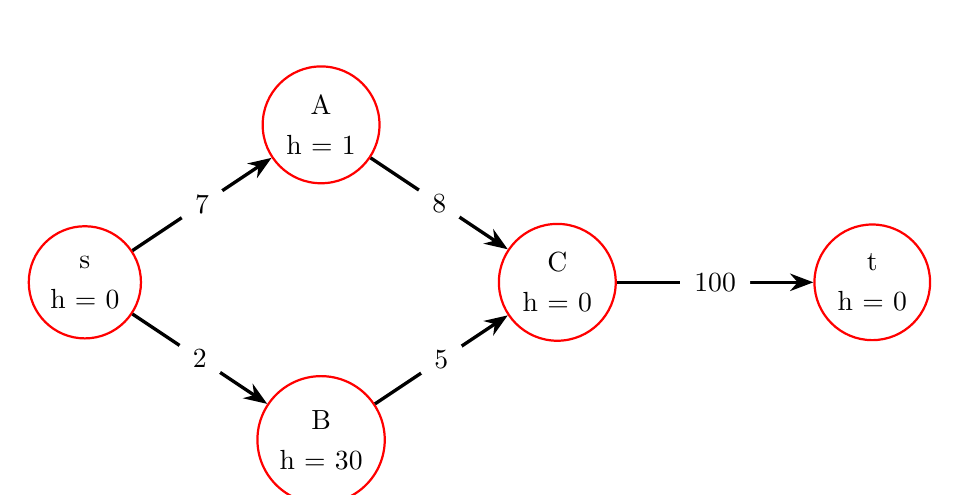
\begin{tikzpicture}
		\begin{scope}[every node/.style={circle,thick,draw=red, align=center}]
			\node (S) at (0,0) {s\\h = 0};
			\node (A) at (3,2) {A\\h = 1};
			\node (B) at (3,-2) {B\\h = 30};
			\node (C) at (6,0) {C\\h = 0};
			\node (T) at (10,0) {t\\h = 0};
		\end{scope}
		\begin{scope}[>={Stealth[black]},
			every node/.style={fill=white,circle},
			every edge/.style={draw,very thick}]
			\path [->] (S) edge node{$7$} (A);
			\path [->] (S) edge node{$2$} (B);
			\path [->] (A) edge node{$8$} (C);
			\path [->] (B) edge node{$5$} (C);
			\path [->] (C) edge node{$100$} (T);
		\end{scope}
	\end{tikzpicture}
\end{center}
After first iteration (remove s), The node in the \(fringe\) should be
$$
	A(g = 7, f = 8, prev = s), B(g = 2, f = 32, prev = s)
$$
Therefore, in the next iteration, both \textit{A* graph search} and \textit{A*-CSCS} will expand \(A\) and the \(fringe\) shoule be
$$
	C(g = 15, f = 15, prev = A), B(g = 2, f = 32, prev = s)
$$
Next, both the algorithm will expand \(C\), and the \(fringe\) is
$$
	B(g = 2, f = 32, prev = s), t(g = 115, f = 115)
$$
After that, both the alogrithm will expand \(B\), and the \(fringe\) is
$$
	C(g = 7, f = 7, prev = B), t(g = 115, f = 115)
$$
At this point, \textit{A* graph search} will not expand \(C\) because it's in \(closed\), but \textit{A*-CSCS} will expand \(C\) because \(g = 7 < g' = 15\) in \(closed\).\\
Therefore, \textit{A*-CSCS} may expand more nodes than \textit{A* graph search}
\pagebreak
\begin{Q}
	the A*-CSCS algorithm with a consistent heuristic will expand at most as many nodes as A* graph search.
\end{Q}
Yes.\\
(Please refer to the notations on the top of this section and the proof of \textbf{Lemma 1} in Q8.)\\
We will prove this by showing that with a consistent heuristic, if a node \(n\) is in $closed$, then \(\hat g(n) = g(n)\). We will prove this by contradiction.\\
\textbf{Lemma 2:}\\
With a consistent heuristic, if a node \(n\) is in $closed$, then \(\hat g(n) = g(n)\).\\
\textbf{Proof:}\\
Consider the graph \(G_s\) just before closing \(n\), suppose that \(COST[n] = \hat g(n) > g(n)\). There exist an optimal path \(P\) from \(s\) to \(t\). By \textbf{Lemma 1 (in Q8)}, there exists a node \(n'\) on P in \(fringe\) with \(COST[n'] = \hat g(n') = g(n')\). If \(n' = n\), then by contradiction, we have proved the lemma. Otherwise,
\begin{align*}
	g(n)                  & = g(n') + h(n', n)                  \\
	                      & = \hat g(n') + h(n', n)             \\
	\hat g(n)             & > g(n)                              \\
	\hat g(n)             & > \hat g(n') + h(n', n)             \\
	\hat g(n) + \hat h(n) & > \hat g(n') + h(n', n) + \hat h(n) \\
\end{align*}
Since the heuristic is consistent
$$
	\hat h(n) + h(n', n) \ge \hat h(n')
$$
Therefore
\begin{align*}
	\hat g(n) + \hat h(n) & > \hat g(n') + \hat h(n') \\
	\hat f(n) > \hat f(n')
\end{align*}
This is contradict to the \(A*\) strategy that \(A*\) always select node with smaller \(\hat f\) for expansion. The \(A*-CSCS\) should expand \(n'\) rather than \(n\) at this stage.\\
Therefore, with a consistent heuristic, if a node \(n\) is in $closed$, then \(\hat g(n) = g(n)\).\\
\textbf{End of proof (Lemma 2)}\\
By lemma 2, we know that if a node is in \(closed\), no more attenption can give a cost less than the cost recorded in \(closed\), since the recorded cost is already optimal.\\
This is means \textit{A*-CSCS} with consistent heuristic will never expand a node again in \(closed\). This is equal to \textit{A* graph search} that will never expand a node in \(closed\). Therefore, the \textit{A*-CSCS} with a consistent heuristic will expand at most as many nodes as \textit{A* graph search}.
\pagebreak
\end{document}